\chapter{Implementation}
In the previous chapter we discussed some of the mathematical and technical details of the project. Based on the information provided in those sections on reinforcement learning and deep learning, this section will discuss the implementation details. Although this project was primarily a research project into the details of reinforcement learning, it does contain a significant software engineering aspect as such this section will also include some code listing and system architecture diagrams.

\section{Environment}
\subsection{OpenAI Gym}
Referring back to Section \ref{dsgn:sec:rl}, reinforcement learning is based upon a simple data flow between the agent (the thing that takes actions) and the environment (the system that produces a state and reward) which is shown diagramatically in Figure \ref{fig:rl-diagram}.

OpenAI Gym provides a well-developed API that interats with the Arcade Learning Environment (ALE) which is used for emulating Atari 2600 games The ALE was developed to support reinforcement researchers to develop agents for Atari\cite{bellemare13arcade}\cite{machado18arcade}. Additionally, OpenAI Gym provides emulation for robotics simulations and text-based environments, however, these were not used in this project. In order to emulate the Atari 2600 console, Gym provides a Python API for ALE, which then uses the Stella\footnote{\href{https://stella-emu.github.io/}{Stella} is a Atari 2600 emulator released under a GNU General Public License for multiple platforms} emulator which actually executes the Atari games on the machine \cite{brockman2016openai}.

The code listing \ref{code:basic-gym} shows the basic API used in order to step through the environment. The agent is initalised first which contains the code for optimising the neural network for predicting the actions based on raw observations. Gym offers the function \mintinline{python}{step(action)} which will update the environment, taking the action provided, and returns a new observation, reward, done signal, and any additional information.

During the experiments performed for this project, the number of timesteps was fixed, with each episode lasting a variable number of timesteps depending on the game. For example, Pong would last an average of 1000 timesteps, whereas Breakout would be around 300 timesteps. This difference was since we considered an episode finished when the agent lost a single life, not when all five lives are lost (as is the standard in the games tested in this project).

During the initial prototyping phase of the project, the environments would be ran for a short time, around 100,000 timesteps, this is in comparison to the finnal evaluation in which we ran the environment for 10 million timesteps. This was primarily since after 100k steps, one could identify is the agent was beginning to improve.

\begin{code}
  \captionof{listing}{Training an agent with OpenAI Gym}
  \label{code:basic-gym}
  \begin{minted}[
    mathescape,
    linenos,
    numbersep=5pt,
    frame=lines,
    framesep=2mm
  ]{python}
import gym
env = gym.make("Pong-v0")
observation = env.reset()

agent = Agent()

for _ in range(1000):
  # Draw the environment in the UI
  env.render()

  # Predict the next action, based on the observation
  action = agent.step(observation)

  # Update environment, taking the action
  # Get a new observation and reward
  observation, reward, done, info = env.step(action)

  if done:
    observation = env.reset()
env.close()
\end{minted}
\end{code}

\section{Agent}
This section will provide implementation details for the agent, how it is trained and motivate the choice of the hyperparamters used during training and evaluation. The section will be split into sections, convering the different aspects of the agent, convolutional layers for handling the raw pixel input, and the fully-connected network for predicting the Q-values of each action.

\subsection{CNN}
The convolutional will be described in this section, it is also shown diagramatically in Figure \ref{fig:project-dqn}. First, from the emulator, we recieve frames with a size of 210x160 pixels. Since the project uses a GPU implementation for performing convolution, we require a square input to the network. As such, each frame is downsampled to 84x84 pixels using a function $\phi(\cdot)$ performing a bilinear interpolation.

Next, we construct a processed frame history ($\phi(s_{t-3}), \phi(s_{t-2}), \phi(s_{t-1}), \phi(s_t)$), the past four frames are processed using the function $\phi(\cdot)$. We briefly mentioned this in Section \ref{dsgn:sec:markov-prop} in which we referred to this concept as a \textit{``frame-stack''} the past $k$ frames.

The first convolutional layer performs a convolution of 32 20x20 filters, each with a stride of 4, to the input layer. The second layer then convolves 64 9x9 filters of stride 2. Next, the third layer convolves 64 7x7 filters of stride 1, producing the final output before the fully-connected network. The output from the last layer is flattened to a vector of 3136 nodes which is fully-connected to 256 ReLU units. Finally, we have between 4 and 6 outputs (depending on the game) with contain the predicted Q-values for each action in the action space for the environment. This architecture was kept the same for all the Atari games during the evaluation of this project.

\begin{figure}[htbp]
  \centering
  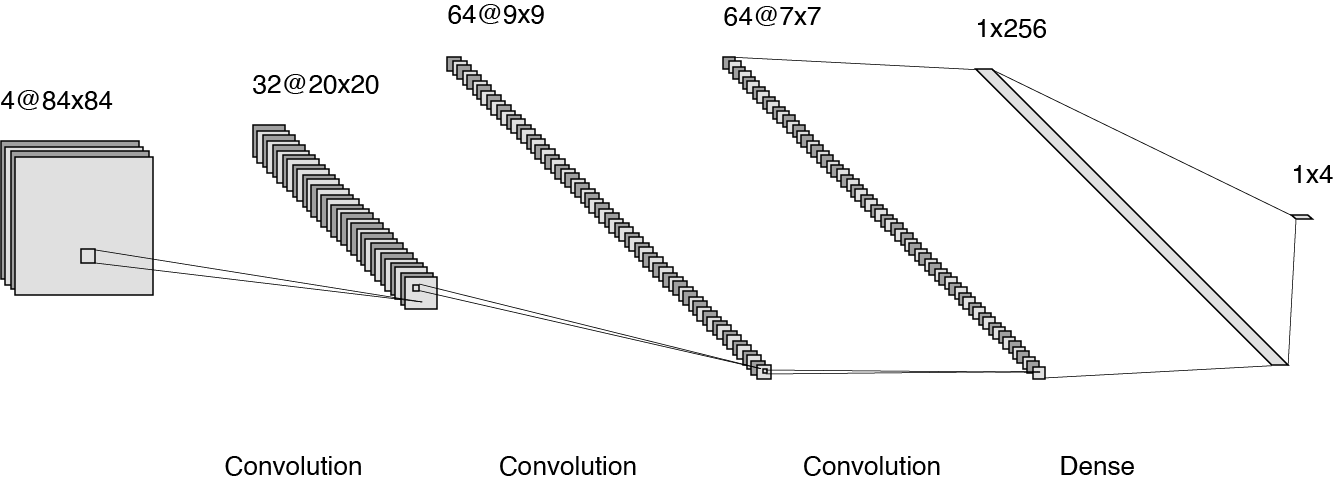
\includegraphics[width=0.75\textwidth]{chapters/chapter4/images/cnn.png}
  \caption{DQN Architecture
    \label{fig:project-dqn}
  }
\end{figure}

\subsection{DQN}

\section{Visualisation}